\documentclass{classrep}
\usepackage[utf8]{inputenc}


\studycycle{Informatyka, studia dzienne, inż I st.}
\coursesemester{V}
\coursename{Obliczenia naukowe}
\courseyear{2017/2018}
\courseteacher{dr hab. Paweł Zieliński}
\coursegroup{czwartek TN, 11:15}

\author{
  \studentinfo{Agata Jasionowska}{229726}
}

\title{Laboratorium \ppauza Lista 3}
\begin{document}

\maketitle

\section{Zadanie 1}
	\subsection{Opis problemu}
		Implementacja funkcji rozwiązującej równanie $f(x)=0$ metodą bisekcji.
	
	\subsection{Opis rozwiązania}
		Zastosowanie metody bisekcji wymaga spełnienia pewnych założeń:
		\begin{enumerate}[1.]
			\item funkcja $f(x)$ jest ciągła w przedziale domkniętym $[a,b]$,
			\item funkcja przyjmuje różne znaki na końcach przedziału $f(a)f(b)<0$.
		\end{enumerate}
		
		Przebieg algorytmu dla tej metody jest następujący:
		\begin{enumerate}
			\item Jeżeli funkcja $f$ nie zmienia znaku w przedziale $[a,b]$ --- zwrócenie informacji o błędzie;
			\item Dopóki $|a-b|>epsilon$, obliczenie $x=\dfrac{a+b}{2}$;
			\item Jeżeli $f(x)=0$ to zwrócenie $x$ jako rozwiązania;
			\item Obranie nowego przedziału ($[a,x]$ lub $[b,x]$), w którym funkcja zmienia znak na przeciwny i powrót do 2.
		\end{enumerate}	
	
		\begin{algorithm}[!htbp]
    			\SetKwInOut{Input}{Input}
    			\SetKwInOut{Output}{Output}
    			
    			\SetKwData{R}{r}
			\SetKwData{Err}{err}
			\SetKwData{V}{v}
			\SetKwData{Valuer}{v}
			\SetKwData{Valuea}{fa}
			\SetKwData{Valueb}{fb}
			\SetKwData{It}{it}
			\SetKwData{Middle}{e}

    			\underline{mbisekcji} ($f,~a,~b,~delta,~epsilon$)\;
		    \Input{
		    			$f$ - funkcja $f(x)$ zadana jako anonimowa funkcja,\\
		    			$a,b$ - końce przedziału początkowego,\\
		    			$delta, epsilon$ - dokładność obliczeń}
		    \Output{
		    			(\R,~\V,~\It,~\Err), gdzie: \\
		    			$\R$ - przybliżenie pierwiastka równania $f(x) = 0$, \\
		    			$\V$ - wartość $f(\R)$, \\
		    			$\It$ - liczba wykonanych iteracji, \\
		    			$\Err$ - sygnalizacja błędu: \\
		    				\quad $0$ - brak błędu, \\
		    				\quad $1$ - funkcja nie zmienia znaku w przedziale $[a,b]$.
		    	}
		    \R $\leftarrow 0$\;
		    \Valuer $\leftarrow 0$\;
		    	\Valuea $\leftarrow f(a)$\;
		    	\Valueb $\leftarrow f(b)$\;
		    	\Middle $\leftarrow b - a$\;
		    	\It $\leftarrow 0$\;
		    \If{$sgn(\Valuea) = sgn(\Valueb)$} {
		    		\Err $\leftarrow 1$\;
		    		\KwRet $(\R,~\Valuer,~\It,~\Err)$\;
		    	}
		    	\While{\Middle $> epsilon$} {
		    		\It $\leftarrow \It + 1$\;
    				\Middle $\leftarrow \Middle / 2$\;
    				\R $\leftarrow a + \Middle$\;
    				\Valuer $\leftarrow f(\R)$\;
    				\If{$|\Middle| < delta$ OR $|\Valuer| < epsilon$} {
    					\KwRet $(\R,~\Valuer,~\It,~\Err)$\;
    				}
    				\eIf{$sign(\Valuer) \neq sign(\Valuea)$} {
    					$b \leftarrow \R$\;
    					\Valueb $\leftarrow \Valuer$\;
    				}
    				{
    				$a \leftarrow \R$\;
    				$\Valuea \leftarrow \Valuer$\;
    				}
    			}
    			\KwRet $(\R,~\Valuer,~\It,~\Err)$\;
    			\caption{Metoda bisekcji}
		\end{algorithm}	
	
\section{Zadanie 2}
	\subsection{Opis problemu}
		Implementacja funkcji rozwiązującej równanie $f(x)=0$ metodą stycznych (Newtona).
		
	\subsection{Opis rozwiązania}
		W przypadku stosowania metody Newtona przyjmuje się kilka założeń co do danej funkcji $f$:
		\begin{enumerate}[1.]
			\item w przedziale domkniętym $[a,b]$ znajduje się dokładnie jeden pierwiastek,
			\item funkcja przyjmuje różne znaki na końcach przedziału $f(a)f(b)<0$,
			\item pierwsza i druga pochodna $f$ mają stały znak w tym przedziale.
		\end{enumerate}
		
		Przebieg tej metody jest następujący:
		\begin{enumerate}
			\item Za $x_1$ przyjmowany jest punkt przecięcia stycznej wyprowadzonej dla $x_0$ z osią \texttt{OX};
			\item Dopóki nie osiągnięto wymaganego przybliżenia, $x_0 = x_1$;
			\item Kolejne przybliżenie obliczane jest ze wzoru: $x_1 = x_0-\dfrac{f(x_0)}{pf(x_0)}$, powrót do kroku 2;
			\item Jeżeli $f(x_0)>epsilon$ zwracany jest błąd, w przeciwnym przypadku rozwiązaniem jest $x_0$.
		\end{enumerate}	
	
		\begin{algorithm}[!htbp]
			\SetKwData{R}{r}
			\SetKwData{Err}{err}
			\SetKwData{Valuer}{v}
			\SetKwData{V}{v}
			\SetKwData{It}{it}
			\SetKwData{X}{x}
			
    			\SetKwInOut{Input}{Input}
    			\SetKwInOut{Output}{Output}

    			\underline{mstycznych} $(f,~pf,~x_0,~delta,~epsilon,~maxit)$\;
		    \Input{
		    			$f,~pf$ - funkcja $f(x)$ oraz $f'(x)$ zadane jako anonimowe funkcje,\\
		    			$x_0$ - przybliżenie początkowe,\\
		    			$delta,~epsilon$ - dokładność obliczeń,\\
		    			$maxit$ - maksymalna dopuszczalna liczba iteracji
		    			}
		    \Output{
		    			(\R,~\V,~\It,~\Err), gdzie: \\
		    			\R~ - przybliżenie pierwiastka równania $f(x) = 0$, \\
		    			\V~ - wartość $f(\R)$, \\
		    			\It~ - liczba wykonanych iteracji, \\
		    			\Err~ - sygnalizacja błędu: \\
		    				\quad $0$ - metoda zbieżna, \\
		    				\quad $1$ - nie osiągnięto wymaganej dokładności w $maxit$ iteracji, \\
		    				\quad $2$ - pochodna bliska zeru.
		    	}
		    	\R $\leftarrow x_0$\;
		    	\Err $\leftarrow 0$\;
		    	\Valuer $\leftarrow f(\R)$\;
		    	\It $\leftarrow 0$\;
		    \If{$|pf(\R)| < epsilon$} {
		    		\Err $\leftarrow 2$\;
		    		\KwRet $(\R,~\Valuer,~\It,~\Err)$\;
		    	}
		    	\For{\It $\gets 1$ \KwTo $maxit$} {
		    		\X $\leftarrow \R - (\Valuer / pf(\R))$\;
		    		\Valuer $\leftarrow f(\X)$\;
		    		\If{$|\R - \X| < delta$ or $|\Valuer| < epsilon$} {
		    			\R $\leftarrow \X$\;
		    			\KwRet $(\R,~\Valuer,~\It,~\Err)$\;
		    		}
		    		\R $\leftarrow \X$\;
    			}
    			\If{$|\Valuer| > epsilon$} {
    				\Err $\leftarrow 1$\;
    			}
    			\KwRet $(\R,~\Valuer,~\It,~\Err)$\;
    			\caption{Metoda stycznych}
		\end{algorithm}	
	
\section{Zadanie 3}
	\subsection{Opis problemu}
		Implementacja funkcji rozwiązującej równanie $f(x)=0$ metodą siecznych(Eulera).
	
	\subsection{Opis rozwiązania}		
		Dla metody siecznych przyjmuje się kilka założeń co do funkcji $f$:
		\begin{enumerate}[1.]
			\item $f$ jest ciągła,
			\item w przedziale domkniętym $[a,b]$ pierwsza pochodna jest różna od zera,
			\item funkcja przyjmuje różne znaki na końcach przedziału $f(a)f(b)<0$.
		\end{enumerate}
		
		Przebieg tej metody jest następujący:
		\begin{enumerate}
			\item Obliczane są wartości $f_1=f(x_1)$ oraz $f_2=f(x_2)$;
			\item Dopóki nie osiągnięto wymaganej liczby iteracji, $x_0=x_1-f_1 \cdot \dfrac{x_1-x_2}{f_1-f_2}$, $f_0=f(x_0)$;
			\item Jeżeli $|x_1-x_2|<epsilon$, zwrócenie $x_0$ i zakończenie działania;
			\item Zamiana parametrów i wartości funkcji odpowiednio dla $x_2 \leftarrow x_1$ oraz $x_1 \leftarrow x_0$, powrót do kroku 2.
		\end{enumerate}
		
		\begin{algorithm}[!htbp]
			\SetKwData{A}{a}
			\SetKwData{B}{b}
			\SetKwData{R}{r}
			\SetKwData{Err}{err}
			\SetKwData{V}{v}
			\SetKwData{Valuea}{fa}
			\SetKwData{Valueb}{fb}
			\SetKwData{It}{it}
			\SetKwData{S}{s}
    			\SetKwInOut{Input}{Input}
    			\SetKwInOut{Output}{Output}
    			\SetKwInOut{OR}{OR}

    			\underline{msiecznych} $(f,~x_0,~x_1,~delta,~epsilon,~maxit)$\;
		    \Input{
		    			$f$ - funkcja $f(x)$ zadana jako anonimowa funkcja,\\
		    			$x_0,~x_1$ - przybliżenia początkowe,\\
		    			$delta,~epsilon$ - dokładność obliczeń,\\
		    			$maxit$ - maksymalna dopuszczalna liczba iteracji
		    			}
		    \Output{
		    			(\R,~\V,~\It,~\Err), gdzie: \\
		    			\R~ - przybliżenie pierwiastka równania $f(x) = 0$, \\
		    			\V~ - wartość $f(\R)$, \\
		    			\It~ - liczba wykonanych iteracji, \\
		    			\Err~ - sygnalizacja błędu: \\
		    				\quad $0$ - metoda zbieżna, \\
		    				\quad $1$ - nie osiągnięto wymaganej dokładności w $maxit$ iteracji.
		    	}
		    	\A $\leftarrow x_0$\;
		    	\B $\leftarrow x_1$\;
		    	\Valuea $\leftarrow f(\A)$\;
		    	\Valueb $\leftarrow f(\B)$\;
		    	\It $\leftarrow 0$\;
		    \Err $\leftarrow 0$\;
		    	
		    	\For{\It $\gets 1$ \KwTo $maxit$} {
		    		\If{$|\Valuea| > |\Valueb|$} {
		    			$swap(\A, \B)$\;
		    			$swap(\Valuea, \Valueb)$\;
		    		}
		    		\S $\leftarrow (\B - \A) / (\Valueb - \Valuea)$\;
		    		\B $\leftarrow \A$\;
		    		\Valueb $\leftarrow \Valuea$\;
		    		
		    		\A $\leftarrow \A - (\Valuea \cdot \S)$\;
		    		\Valuea $\leftarrow f(\A)$\;		    		
		    		
    				\If{$|\Valuea| < epsilon$ \texttt{OR} $|\B - \A| < delta$} {
    					\KwRet $(\A,~\Valuea,~\It,~\Err)$\;
    				}
    			}
    			\If{$|\Valuea| > epsilon$ \texttt{AND} $|\B - \A| > delta$} {
    				\Err $\leftarrow 1$\;
    			}
    			\KwRet $(\A,~\Valuea,~\It,~\Err)$\;
    			\caption{Metoda siecznych}
		\end{algorithm}	
	
\section{Zadanie 4}
	\subsection{Opis problemu}
		Przy użyciu metod zaprogramowanych w poprzednich zadaniach wyznaczenie pierwiastka równania $sin{x}-(\dfrac{1}{2}x)^2=0$ dla poniższych danych:
		\begin{enumerate}[1.]
			\item Metodą bisekcji z przedziałem początkowym $[1.5,2],~\delta=\dfrac{1}{2}10^{-5},~\epsilon=\dfrac{1}{2}10^{-5}$;
			\item Metodą Newtona z przybliżeniem początkowym $x_0=1.5,~\delta=\dfrac{1}{2}10^{-5},~\epsilon=\dfrac{1}{2}10^{-5}$;
			\item Metodą siecznych z przybliżeniem początkowym $x_0=1,~x_1=2,~\delta=\dfrac{1}{2}10^{-5},~\epsilon=\dfrac{1}{2}10^{-5}$.
		\end{enumerate}
		
	\subsection{Opis rozwiązania}
		Zastosowanie funkcji utworzonych w zadaniach 1-3.
	
	\subsection{Wyniki}
		Uzyskane rezultaty widoczne są w Tabeli \ref{table:1}.
		
		\begin{table}[!hpbt]
        		\centering
        		\footnotesize
			\sisetup{
				table-number-alignment = right,
				table-figures-integer = 1,
				table-figures-decimal = 16,
				table-figures-exponent = 1
			}
			\begin{tabular}{lSSl} \toprule
				{podpunkt} & {$x_0$} & {$f(x_0)$} & {liczba iteracji}\\ \midrule
				$1.$ & 1.9337539672851562 & -2.7027680138402843e-7 & 16 \\ 
	 			$2.$ & 1.933753779789742 & -2.2423316314856834e-8 & 4 \\
	 			$3.$ & 1.9337509005356321 & 3.783706985283075e-6 & 4 \\ \bottomrule
	 		\end{tabular}
	 		\caption{$sin{x}-(\dfrac{1}{2}x)^2=0$ dla danych z zadania}
			\label{table:1}
		\end{table}	
		
	\subsection{Wnioski}
		Funkcja metody biekcji wykonała znacznie więcej iteracji, bo aż 17. Jednak w efekcie końcowym to ona zwróciła wynik z najmniejsza dokładnością. 
		O wiele lepiej radzą tu sobie funkcje siecznych oraz stycznych, osiągając wymaganą dokładność już po 4 iteracjach. Jako zwycięzcę wytypować można metodę Newtona, bowiem osiągnęła ona najdokładniejszy wynik.
		
\section{Zadanie 5}
	\subsection{Opis problemu}
		Wyznaczenie przy pomocy metody bisekcji wartości zmiennej $x$, dla której następuje przecięcie wykresów funkcji $y=3x$ oraz $y=\exp^x$ dla dokładności $\delta=10^{-4}$, $\epsilon=10^{-4}$.
	
	\subsection{Opis rozwiązania}
		W celu rozwiązania zadania zastosowano metodę \texttt{mbisekcji} utworzoną w zadaniu 1.
		Aby określić miejsce przecięcia zadanych funkcji należy znaleźć taki punkt, dla którego przyjmują one identyczną wartość dla tego samego argumentu, czyli $f(x)=3x-\exp^x$. 	\\
		 Najprostszym sposobem określenia przedziałów początkowych będzie analiza wykresu obu funkcji. Z Rysunku \ref{fig:1} wywnioskować można, iż poszukiwane wyniki znajdą się w przedziałach $[0.0,1.0]$ oraz $[1.0,2.0]$.
		
		\begin{figure}[!htbp]
			\centering
			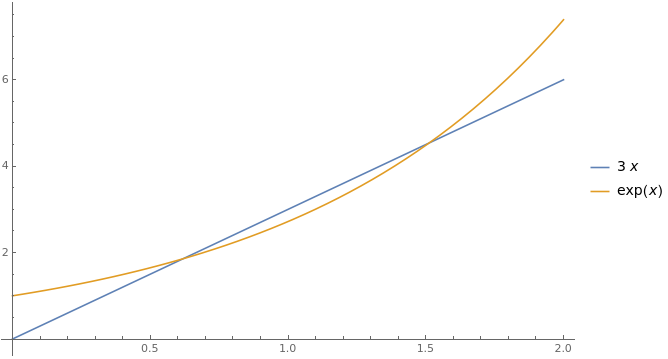
\includegraphics[width=0.5\textwidth]{zadania/plot51.png}
  			\caption{Wykres funkcji w programie Mathematica.}
  			\label{fig:1}
		\end{figure}	
		
	\subsection{Wyniki}
		Poniższa tabela prezentuje otrzymane rozwiązania:
		\begin{table}[!hpbt]
        		\centering
        		\footnotesize
			\sisetup{
				table-number-alignment = right,
				table-figures-integer = 1,
				table-figures-decimal = 12
			}
			\begin{tabular}{lSl} \toprule
				{przedział} & {$x$} & {liczba iteracji}\\ \midrule
				$[0.0,1.0]$ & 0.619140625 & $9$ \\ 
	 			$[1.0,2.0]$ & 1.5120849609375 & $13$ \\ \bottomrule
	 		\end{tabular}
	 		\caption{...}
			\label{table:2}
		\end{table}	
		
	\subsection{Wnioski}
		Ważnym czynnikiem wpływającym na pomyślne znalezienie pierwiastków funkcji metodą bisekcji jest umiejętny dobór przedziału początkowego. Należy zwrócić uwagę, iż w tym przypadku uruchomienie jej dla przedziału $[0.0,2.0]$ zwróci błąd związany z niezmiennością znaku. Jednak po wyszczególnieniu $[0.0,1.0]$ i $[1.0,2.0]$ znalezienie miejsc zerowych $f(x)$ nie nastręcza problemów. Pomocne w czynności wyboru startowego przedziału może być na przykład analiza wykresu funkcji.
		
\section{Zadanie 6}
	\subsection{Opis problemu}
		Znalezienie pierwiastków funkcji $f_1(x)=exp^{1-x}-1$ oraz $f_2(x)=x\exp^{-x}$ przy pomocy metod: bisekcji, stycznych oraz siecznych z dokładnością obliczeń $\delta=10^{-4}$, $\epsilon=10^{-4}$. Należy zadbać o dobór odpowiedniego przedziału oraz przybliżeń początkowych.
		
	\subsection{Opis rozwiązania}
		W rozwiązaniu zadania zastosowano metody \texttt{mbisekcji}, \texttt{msiecznych} oraz \texttt{mstycznych}, utworzone w zadaniach 1-3.
		Rozpoczęto od przeprowadzenia analizy wykresów (Rysunek \ref{fig:2}) zadanych funkcji w celu określenia trafnych parametrów.
		
		\begin{figure}[!htbp]
			\centering
			\subfloat[1.][$f_1(x)=exp^{1-x}-1$]{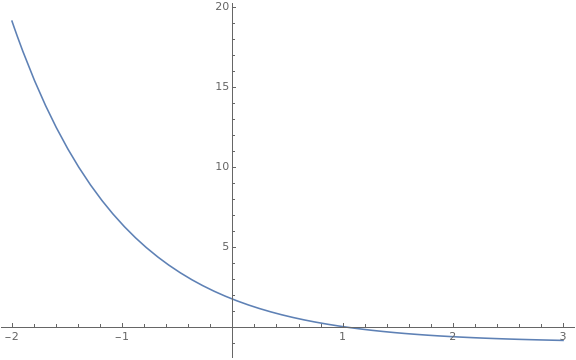
\includegraphics[width=0.5\textwidth]{zadania/plot61.png}} \hfill
			\subfloat[2.][$f_2(x)=x\exp^{-x}$]{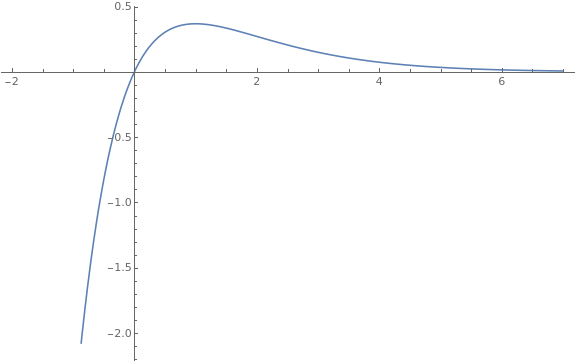
\includegraphics[width=0.5\textwidth]{zadania/plot62.png}}
  			\caption{...}
  			\label{fig:2}
		\end{figure}		
		
	
		\begin{enumerate}[1)]
			\item $f_1(x)$ \\
			Z wykresu z łatwością można odczytać prawidłowe rozwiązanie, jakim jest $x=1.0$.
			Dla metody bisekcji unikano sytuacji, gdy pierwiastek znajduje się w środku przedziału początkowego. Wykonywanie funkcji kończy się wtedy już po pierwszej iteracji, co nie jest interesujące w tym zadaniu.
			Podczas używania metody Newtona należało uważać przy dobieraniu $x_0$, gdyż pochodna dąży do $0$, co jest niepożądane dla tej metody.
			W funkcji metody siecznych wybranie zbyt dużych wartości przybliżeń sprawi, że obliczenia wykonane są na bliskich sobie wartościach i działanie zakończy się szybko ze względu na osiągnięcie założonej precyzji.
			
			\item $f_2(x)$ \\
			Już sam wzór funkcji wskazuje właściwy pierwiastek, czyli $x=0.0$. Podczas używania metody bisekcji ponownie unikano obierania takich przedziałów, że pierwiastek leżał dokładnie w ich połowie. Tym razem jednak wybrano przedział, w którym wartość $0.0$ znajduje się znacznie bliżej środka niż dla funkcji $f_1(x)$. 
		Dla pozostałych dwóch metod zastosowano podobne środki ostrożności co w przypadku funkcji z punktu 1).
		\end{enumerate}
		
		
	\subsection{Wyniki}
		\begin{table}[!hpbt]
        		\centering
        		\footnotesize
			\sisetup{
				table-number-alignment = right,
				table-figures-integer = 1,
				table-figures-decimal = 16,
				table-figures-exponent = 1
			}
			\begin{tabular}{llSSl} \toprule
				{metoda} & {początkowe dane} &{$x$} & {$f(x)$} & {liczba iteracji}\\ \midrule
				bisekcji & $[a,b]=[0.1,1.2]$ & 0.9999938964843748 & 6.103534251789e-6 & $14$ \\ 
	 			stycznych & $x_0=0.3$ & 0.9999999866969493 & 1.3303050661050975e-8 & $4$ \\
	 			siecznych & $x_0=-0.4,~x_1=1.3$ & 1.0000026160714057 & -2.6160679837961e-6 & $7$ \\ 
	 			siecznych & $x_0=-2.0,~x_1=2.0$ & 1.0000063854903036 & -6.385469916381226e-6 & $23$ \\ \bottomrule
	 		\end{tabular}
	 		\caption{$f_1(x)=exp^{1-x}-1$.}
			\label{table:3}
		\end{table}
			
		\begin{table}[!hpbt]
        		\centering
        		\footnotesize
			\sisetup{
				table-number-alignment = right,
				table-figures-integer = 1,
				table-figures-decimal = 16,
				table-figures-exponent = 1
			}
			\begin{tabular}{llSSl} \toprule
				{metoda} & {początkowe dane} &{$x$} & {$f(x)$} & {liczba iteracji}\\ \midrule
				bisekcji & $[a,b]=[-0.4,0.7]$ & -4.5776367187399074e-6 & -4.577657673545798e-6 & $16$ \\ 
	 			stycznych & $x_0=0.4$ & -8.878980981560664e-6 & -8.879059818213929e-6 & $4$ \\  	
	 			siecznych & $x_0=-1.0,~x_1=0.3$ & 9.44134425373555e-6 & 9.441255115175028e-6 & $23$ \\
	 			siecznych & $x_0=-0.1,~x_1=0.9$ & 1.10233618098865e-6 & 1.102334965844264e-6 & $6$ \\ \bottomrule
	 		\end{tabular}
	 		\caption{$f_2(x)=x\exp^{-x}$.}
			\label{table:4}			
		\end{table}	
		
		\begin{table}[!hpbt]
        		\centering
        		\footnotesize
			\sisetup{
				table-number-alignment = right,
				table-figures-integer = 1,
				table-figures-decimal = 16,
				table-figures-exponent = 1
			}
			\begin{tabular}{lSSl} \toprule
				{$x_0$} & {$x$} & {$f(x)$} & {liczba iteracji}\\ \midrule
				$1.5$ & 0.9999999810061002 & 1.8993900008368314e-8 & $5$ \\ 
				$2.5$ & 0.9999999710783241 & 2.892167638712806e-8 & $9$ \\
	 			$4.5$ & 0.9999999995278234 & 4.721765201054495e-10 & $21$ \\
	 			$5.0$ & 0.9999996427095682 & 3.572904956339329e-7 & $54$ \\
	 			$7.5$ & 0.9999999573590406 & 4.264096031825204e-8 & $147$ \\
	 			$10.0$ & 0.9999999484165362 & 5.15834650549607e-8 & $401$ \\ \bottomrule
	 		\end{tabular}
	 		\caption{Metoda Newtona dla $f_1(x)=exp^{1-x}-1$ i $x_0\in{(1,\infty)}$.}
			\label{table:5}			
		\end{table}	
		
		\begin{table}[!hpbt]
        		\centering
        		\footnotesize
			\sisetup{
				table-number-alignment = right,
				table-figures-integer = 1,
				table-figures-decimal = 16,
				table-figures-exponent = 1
			}
			\begin{tabular}{lSSl} \toprule
				{$x_0$} & {$x$} & {$f(x)$} & {liczba iteracji}\\ \midrule
				$2.0$ & 0.9999999810061002 & 1.8993900008368314e-8 & $5$ \\ 
				$3.0$ & 0.9999999710783241 & 2.892167638712806e-8 & $9$ \\
	 			$4.0$ & 0.9999999995278234 & 4.721765201054495e-10 & $21$ \\
	 			$5.0$ & 0.9999996427095682 & 3.572904956339329e-7 & $54$ \\
	 			$6.0$ & 0.9999999573590406 & 4.264096031825204e-8 & $147$ \\
	 			$7.0$ & 0.9999999484165362 & 5.15834650549607e-8 & $401$ \\  \bottomrule
	 		\end{tabular}
	 		\caption{Metoda Newtona dla $f_2(x)=x\exp^{-x}$ i $x_0>1$.}
			\label{table:6}			
		\end{table}	

	\subsection{Wnioski}
		Zestawienie wyników z tabel widocznych powyżej pozwala na wyciągnięcie kilku wniosków. Otóż metoda bisekcji nie ma żadnych ograniczeń związanych z przebiegiem zadanej funkcji oraz jej pochodnej (w przeciwieństwie np. do metody Newtona). Niezależnie od przesunięć przedziału względem poprawnego pierwiastka wylicza wynik w tym samym tempie zależnym od wielkości przedziału (ma to sens, gdyż metoda ta polega na sukcesywnym dzieleniu przedziału na pół aż do momentu uzyskania takiego o satysfakcjonująco małym rozmiarze). Metoda stycznych najlepiej radzi sobie z wyznaczaniem pierwiastka, gdy kluczem jest szybkość --- ze wszystkich badanych metod zwracała ona rozwiązanie po najmniejszej liczbie wykonanych iteracji. Nie oznacza to jednak, że jest najlepszym wyborem w każdej sytuacji --- należy brać pod uwagę jej ograniczenia, nakładane przez konieczność obliczania pochodnej funkcji.  \\
	
		TEMP NOTES:	 \\
		Wnioski dla wyników metody Newtona przy szczególnych argumentach!!!		
		Dla pierwszego: nie udało się wyliczyć dla $x_0=8$ - wciąż niewystarczająca była obrana liczba iteracji wynosząca $it=10000000000$.
		Dla drugiego: podanie argumentu początkowego $x_0=1.0$ powodowało zwrócenie błędu --- pochodna bliska wartości $0.0$.
		
\end{document}
